\documentclass[../main.tex]{subfiles}
\usepackage{slashed}
\usepackage[table]{xcolor}
\usepackage{hhline}
\usepackage{lipsum}

\let\Bbbk\relax
\usepackage{amsmath}
\usepackage{amsfonts}
\usepackage{simpler-wick}

\begin{document}
\setchapterimage[6.5cm]{images_ch4/dyson.png}
\setchapterpreamble[u]{\margintoc}
\chapter[Rinormalizzazione Perturbativa della QED]{Rinormalizzazione Perturbativa della QED\footnote{Freedman Dyson e la rinormalizzazione, rappresentazione artistica da \href{https://youtu.be/qe7atm1x6Mg}{Quanta Magazine}.}}
\labch{PR_QED}
\fboxsep =1pt % separazione per i box

\section{Lagrangiana e contro-termini}
In luce di quanto discusso nel capitolo precedente riscriviamo la Lagrangiana di QED nella seguente forma:
\begin{equation}
    \mathscr L_B = -\frac{1}{4}\bigl( \partial^\mu A_B^\nu - \partial^\nu A_B^\mu \bigr)^2 + \bar \psi_B\bigl( i\gamma^\mu\partial_\mu - m_B + e_B\slashed{A}_B\bigr)\psi_B
    \label{eq:bare_lagrangian_QED}
\end{equation}
nota come \textbf{Lagrangiana nuda} (dall'inglese “\textit{bare}”).

Questa non è altro che la Lagrangiana originale (\ref{eq:QED_lagrangian}), l'unica differenza risiede nell'indicare esplicitamente la natura non fisica dei parametri “$e$” ed “$m$”, che prendono quindi il pedice “$B$” e sono detti \textbf{parametri nudi}.
Inoltre abbiamo introdotto lo stesso pedice anche per i campi, d'altronde abbiamo visto nella nota \ref{note:field_rescaling} come il rescaling dei campi non modifichi la fisica della teoria.
\marginnote{A livello concettuale, questo è un grande passo avanti. Stiamo praticamente dicendo che i parametri ed i campi nella Lagrangiana sono parametri liberi e non fissati!}
Adesso modifichiamo nuovamente questa scrittura passando per i seguenti step:
\begin{enumerate}
    \item[1)] \textbf{Introduciamo i campi rinormalizzati}, indicati dal pedice “$R$”, definendo:
    \[ \psi_B\equiv\sqrt{Z_2}\psi_R ~,~ A^\mu_B \equiv \sqrt{Z_3}A^\mu_R\]
    dove $Z_{2,3}$ sono gli stessi residui dei propagatori vestiti che abbiamo già incontrato.

    Come conseguenza di questa definizione, otteniamo la seguente relazione:
    \begin{align*}
       \underbrace{ \begin{tikzpicture}[baseline=\plusheight]
            \begin{feynman}[] % dressed electron propagator diagram
                \vertex[dot, label={$p$}] (a) at (-1,0) {} ;
                \vertex[large, blob] (m) at (0,0) {};
                \vertex[dot] (b) at (1,0) {};
                \diagram*[small] {
                    (a)--[fermion] (m) -- (b)
                    };
            \end{feynman}
        \end{tikzpicture} 
        =
        \langle \Omega | T\bigl[\psi_B(x_1) \bar \psi_B(x_2) \bigr] | \Omega \rangle }_{\substack{\text{è lo stesso oggetto che abbiamo già calcolato,}\\\text{abbiamo solo rinominato la Lagrangiana}}}\equiv Z_2 \langle \Omega | T\bigl[\psi_R(x_1) \bar \psi_R(x_2) \bigr] | \Omega \rangle
    \end{align*}
    Invertendo in funzione del propagatore “rinormalizzato” otteniamo:
    \[
    \langle \Omega | T\bigl[\psi_R(x_1) \bar \psi_R(x_2) \bigr] | \Omega \rangle = \frac{1}{Z_2}\langle \Omega | T\bigl[\psi_B(x_1) \bar \psi_B(x_2) \bigr] | \Omega \rangle
    \]
    Il rescaling, quindi, forza il residuo del propagatore del campo rinormalizzato $\psi_R$ ad essere $i$.
    
    La Lagrangiana diventa:
    \begin{equation}
        \mathscr L_B = -\frac{Z_3}{4}\bigl( \partial^\mu A_R^\nu - \partial^\nu A_R^\mu \bigr)^2 + Z_2\bar \psi_R\bigl( i\gamma^\mu\partial_\mu - m_B\bigr)\psi_R + e_B Z_2 \sqrt{Z_3}\bar\psi_R\slashed{A}_R\psi_R
        \label{eq:bare_lagrangian_QED_v2}
    \end{equation}

    \item[2)] \textbf{Introduciamo la rinormalizzazione di massa $Z_m$ e di carica $Z_e$} definendo:
    \[ m_B \equiv Z_m m_R ~,~ e_B \equiv Z_e e_R\]

    La Lagrangiana a questo punto diviene (tralasciando per facilità di notazione il pedice “$R$” nel caso dei campi):

    \[\mathscr L_B = -\frac{Z_3}{4}\bigl( \partial^\mu A^\nu - \partial^\nu A^\mu \bigr)^2 + iZ_2 \bar\psi\slashed\partial \psi - Z_2Z_m m_R\bar\psi\psi +  Z_1 e_R\bar\psi\slashed{A}\psi\]
    dove abbiamo anche definito $Z_1=Z_2 \sqrt{Z_3}Z_e$

    \item[3)] \textbf{Ridefiniamo le costanti di rinormalizzazione}, ovvero $Z_1$, $Z_2$, $Z_3$ e $Z_m$ nel seguente modo: \marginnote{\textbf{Attenzione:} non stiamo aggiungendo nuovi parametri! Stiamo ridefinendo quelli già introdotti in maniera da rendere l'approccio perturbativo più facile da sviluppare.}
    \begin{align*}
        &Z_1 \equiv (1 + \delta_1) ~~~~~ Z_2 Z_m m_R \equiv m_R +\delta_m \\
        &Z_2 \equiv (1 + \delta_2) \\
        &Z_3 \equiv (1 + \delta_3) 
    \end{align*}
    Sostituiamo il tutto nella Lagrangiana, e senza troppa difficoltà otteniamo:
    \begin{align*}
        \mathscr L_B = &-\frac{1}{4} F_{\mu\nu} F^{\mu\nu} + i\bar\psi\slashed\partial \psi - m_R\bar\psi\psi + e_R\bar\psi\slashed{A}\psi \\
         & -\frac{\delta_3}{4} F_{\mu\nu} F^{\mu\nu}  + i\delta_2 \bar\psi\slashed\partial \psi - \delta_m \bar\psi\psi + \delta_1 e_R\bar\psi\slashed{A}\psi
    \end{align*}
\end{enumerate}

In sintesi possiamo scrivere la nostra Lagrangiana nuda come somma di due Lagrangiane distinte, una detta “rinormalizzata” e una detta “dei contro-termini” (dove i \textbf{contro-termini} sono i parametri $\delta_i$):
\begin{equation}
    \boxed{
    \begin{aligned}
    \mathscr L_B = \mathscr L_R + &\mathscr L_{ct}\\
    \mathscr L_R = -\frac{1}{4} F_{\mu\nu} F^{\mu\nu} + i\bar\psi\slashed\partial \psi &- m_R\bar\psi\psi + e_R\bar\psi\slashed{A}\psi \\
    \mathscr L_{ct} = -\frac{\delta_3}{4} F_{\mu\nu} F^{\mu\nu}  + i\delta_2 \bar\psi\slashed\partial \psi &- \delta_m \bar\psi\psi + \delta_1 e_R\bar\psi\slashed{A}\psi
    \end{aligned}}
    \label{eq:renormalized+counterterms_lagrangians}
\end{equation}
\begin{nota}
    Ancora una volta, ripetiamo che $\mathscr L_R + \mathscr L_{ct}$ è uguale alla Lagrangiana da cui siamo partiti, abbiamo solo “scritto meglio per il seguito” alcuni termini.
\end{nota}

\section{Regole di Feynman per i contro-termini}
$\mathscr L_R$ ha formalmente la stessa struttura di $\mathscr L_B$. L'unica differenza risiede nella presenza di campi e parametri rinormalizzati, invece dei campi e dei parametri nudi.

Come interpretiamo $\mathscr L_{ct}$? Il modo più conveniente quello è di interpretarla come una nuova Lagrangiana di interazione. Di conseguenza, associamo ad $\mathscr L_{ct}$ nuove regole di Feynman.

\subsection{Regola per $\delta_3$}
\begin{align*}
    \mathscr L_{ct}\supset &-\frac{\delta_3}{4} F_{\mu\nu} F^{\mu\nu} =\\
                           &= -\frac{\delta_3}{2}\bigl(\partial_\mu A_\nu\bigr)\bigl(\partial^\mu A^\nu - \partial^\nu A^\mu\bigr) =\\ \substack{\text{integrando}\\ \text{per parti}}
                           & = +\frac{\delta_3}{2}A^\nu\bigl(g_{\mu\nu}\partial_\rho\partial^\rho - \partial_\mu\partial_\nu \bigr)A^\mu
\end{align*}
Questo operatore corrisponde allo scattering “one-to-one” \marginnote{quando il diagramma è relativo alla “interazione dei contro-termini”, utilizziamo il cerchio con la croce come vertice di interazione.}
\[
\feynmandiagram[horizontal=a to v, layered layout]{
    a[label=below:\rho] --[photon, momentum=\(p\)] v[crossed dot] --[photon, momentum=\(p\)] b[label=below:\sigma]
};
\]
e la regola di Feynman corrispondente può essere calcolata come al solito dall'elemento di matrice corrispondente.

Ci sono due possibili contrazioni: \marginnote{\textbf{Nota:} qui $\lambda$ rappresenta l'elicità del fotone.}
\begin{align*}
i\mathcal{M} = & 
    \wick[positions={+1,-1}]{
    \frac{i\delta_3}{2}\langle p, \c1{\lambda} | \c1{A^{\rho}}\bigl(g_{\rho\sigma}\partial_\alpha\partial^\alpha - \partial_\rho\partial_\sigma \bigr)\c2{A^\sigma} | p, \c2{\lambda} \rangle
    }\\
& + \wick[positions={+1,-1}]{
    \frac{i\delta_3}{2}\langle p, \c1{\lambda} | \c2{A^{\rho}}\bigl(g_{\rho\sigma}\partial_\alpha\partial^\alpha - \partial_\rho\partial_\sigma \bigr)\c1{A^\sigma} | p, \c2{\lambda} \rangle
} \overset{\star}{=}
\end{align*}

La contrazione \( \wick{\c2{A^\sigma} | p, \c2{\lambda} \rangle} = \feynmandiagram[layered layout, small, horizontal=a to b, baseline=\plusheight]{a --[photon] b[dot]}; = \varepsilon^\sigma(p,\lambda)\) tira fuori il tensore di polarizzazione dal campo fotonico, con il c.c. se trattiamo la contrazione con lo stato iniziale.

Il risultato dei due termini è lo stesso, l'unica parte “tricky” del calcolo è dovuta alla presenza dell'operatore di derivata agente sul campo $A^\sigma$.

Adottando la notazione
\[
A^\sigma(x) = \int\frac{d^3\Vec{p}}{(2\pi)^3} \frac{1}{\sqrt{2E_p}} \sum_\lambda \bigl[ a(\Vec{p},\lambda) \varepsilon^\sigma(p,\lambda)e^{-ip\cdot x} + c.c.\bigr]
\]
per calcolo bruto si dimostra che 
\begin{align*}
    &\bigl( g_{\rho\sigma}\partial_\alpha\partial^\alpha - \partial_\rho\partial_\sigma\bigr)\wick{\c2{A^\sigma} | p, \c2{\lambda} \rangle} = \bigl( -g_{\rho\sigma}p^2 + p_\rho p_\sigma\bigr)\varepsilon^\sigma(p,\lambda)\\
    &\wick[positions={-1}]{\langle p, \c1{\lambda}| \bigl( g_{\rho\sigma}\partial_\alpha\partial^\alpha - \partial_\rho\partial_\sigma\bigr)\c1{A^\sigma} } = \bigl( -g_{\rho\sigma}p^2 + p_\rho p_\sigma\bigr){\varepsilon^\sigma}^*(p,\lambda)    
\end{align*}

Di conseguenza, proseguendo il calcolo dell'elemento di matrice:
\begin{align*}
    \overset{\star}{=} \frac{i\delta_3}{2}{\varepsilon^\rho}^*\bigl( -g_{\rho\sigma}p^2 + p_\rho p_\sigma\bigr)\varepsilon^\sigma + \frac{i\delta_3}{2}\bigl( -g_{\rho\sigma}p^2 + p_\rho p_\sigma\bigr){\varepsilon^\sigma}^*\varepsilon^\rho 
\end{align*}
Ricordando che \({\varepsilon^\rho}^*\varepsilon^\sigma = \frac{1}{2}\bigl({\varepsilon^\rho}^*\varepsilon^\sigma + {\varepsilon^\sigma}^*\varepsilon^\rho \bigr)\) troviamo in definitiva:
\[
i\mathcal{M} = {-i\delta_3}\bigl(g_{\rho\sigma}p^2 - p_\rho p_\sigma\bigr){\varepsilon^\rho}^*(p,\lambda)\varepsilon^\sigma(p,\lambda)
\]
La regola che stiamo cercando sarà allora:
\begin{equation}
    \boxed{
    \feynmandiagram[horizontal=a to v, layered layout, baseline=\plusheight]{
    a[label=below:\mu] --[photon, momentum=\(p\)] v[crossed dot] --[photon, momentum=\(p\)] b[label=below:\nu]
    }; \equiv {-i\delta_3}\bigl(g_{\mu\nu}p^2 - p_\mu p_\nu\bigr)}
    \label{eq:delta_3_rule}
\end{equation}

\subsection{Regola per $\delta_2$ e $\delta_m$}

\[
\mathscr L_{ct} \supset  i\delta_2 \bar\psi\slashed\partial \psi - \delta_m \bar\psi\psi 
\]
Estraiamo la regola di Feynman con lo stesso trucco di prima, considerando l'ampiezza del processo one-to-one mediato esattamente da quel termine:
\[
\feynmandiagram[horizontal=a to v, layered layout]{
    a[label=\(p\)] --[fermion] v[crossed dot] --[fermion] b
};
\]

Tale ampiezza risulta essere:
\[i\mathcal{M} = \underbrace{\langle e^-(p,\sigma) |}_{\substack{\text{stato finale}}} i\bar\psi\bigl(i\delta_2\gamma^\mu\partial_\mu -\delta_m\bigr)\psi \underbrace{| e^-(p,\sigma) \rangle}_{\substack{\text{stato iniziale}}}\]

Ricordiamo ora l'espansione del campo di Dirac libero:

\begin{align*}
    \psi = \int \frac{d^3\Vec{k}}{(2\pi)^3} \frac{1}{\sqrt{2E_k}}\sum_s\bigl[ \overbrace{a(\Vec{k},s)u(k,s)e^{-ik \cdot x}}^{\substack{\text{distrugge} \\ \text{la particella}}} + \overbrace{b^\dagger(\Vec{k},s)v(k,s)e^{ik \cdot x}}^{\substack{\text{crea} \\ \text{l'anti-particella}}}\bigr]\\
    \bar \psi = \int \frac{d^3\Vec{k}}{(2\pi)^3} \frac{1}{\sqrt{2E_k}}\sum_s\bigl[ \underbrace{b(\Vec{k},s)\bar v(k,s)e^{-ik \cdot x}}_{\substack{\text{distrugge} \\ \text{l'anti-particella}}} + \underbrace{a^\dagger(\Vec{k},s)\bar u(k,s)e^{ik \cdot x}}_{\substack{\text{crea} \\ \text{la particella}}}\bigr]
\end{align*}

Ne deduciamo che solo una contrazione è possibile, ovvero:
\[
    \wick{
    \langle \c1{e^-(p,\sigma)} |i\c1{\bar\psi}\bigl(i\delta_2\gamma^\mu\partial_\mu -\delta_m\bigr)\c2{\psi} | \c2{e^-(p,\sigma)} \rangle
    }
\]
Tipicamente, queste contrazioni forniscono i seguenti risultati:
\begin{align*}
\wick{\c2{\psi} | \c2{e^-(p,\sigma)} \rangle} = \feynmandiagram[layered layout, small, horizontal=a to b, baseline=\plusheight]{a --[fermion] b[dot]}; = u(p,\sigma)\\
\wick{\langle \c1{e^-(p,\sigma)} |\c1{\bar\psi}} = \feynmandiagram[layered layout, small, horizontal=a to b, baseline=\plusheight]{a[dot] --[fermion] b}; = \bar u(p,\sigma)
\end{align*}
tuttavia noi abbiamo una derivata $\partial_\mu$ che agisce su $\psi$ nel termine proporzionale a $\delta_2$.

Siccome \(\textcolor{Red}{\partial_\mu}\psi = \int \frac{d^3\Vec{k}}{(2\pi)^3} \frac{1}{\sqrt{2E_k}}\sum_s\bigl[ a(\Vec{k},s)u(k,s)\textcolor{Red}{(-ik_\mu)}e^{-ik \cdot x} + b^\dagger(\Vec{k},s)v(k,s)\textcolor{Red}{(ik_\mu)}e^{ik \cdot x}\bigr]\\\) allora 
\[
\wick{\c2{\partial_\mu\psi} | \c2{e^-(p,\sigma)} \rangle} = -ip_\mu u(p,\sigma)
\]

In definitiva, l'ampiezza si scrive

\begin{align*}
i\mathscr M &= i\bar u(p,\sigma) \bigl[i\delta_2\gamma^\mu(-ip_\mu) -\delta_m \bigr]u(p,\sigma) =\\
&= \bar u(p,\sigma) i\bigl(\delta_2\gamma^\mu p_\mu -\delta_m \bigr) u(p,\sigma)
\end{align*}
Da cui segue immediatamente la regola 
\[
\boxed{\feynmandiagram[small, horizontal=a to v, layered layout]{
    a[label=$p$] --[fermion] v[crossed dot] --[fermion] b
}; = i\bigl(\delta_2\slashed p -\delta_m \bigr)}
\]
\subsection{Regola per $\delta_1$}
$\delta_1$ è detto contro-termine di vertice. Infatti il termine della Lagrangiana che lo contiene
\[\mathscr{L}_{ct} \supset \delta_1 e_R \bar\psi\gamma^\mu A_\mu\psi\]
ha la stessa struttura del vertice di QED.

La regola di Feynman associata risulta quindi triviale ed è:
\begin{align*}
    \boxed{\feynmandiagram[horizontal=v to c, layered layout, inline=(c.base)]{
        a --[anti fermion] v[crossed dot] --[anti fermion] b,
        v --[photon]  c,
        {[same layer] a, b},
    }; 
    = i\delta_1e_R\gamma^\mu}
\end{align*}
\begin{nota}
    Commentiamo quanto visto fino ad ora
    \begin{enumerate}
        \item[1)] Non abbiamo aggiunto alcun nuovo termine alla Lagrangiana.
        \item[2)] Abbiamo riorganizzato la Lagrangiana originale avvalendoci della libertà di riscalare i campi e del fatto che i parametri nudi non sono i parametri fisici.
        \item[3)] La Lagrangiana rinormalizzata ha precisamente la stessa struttura di quella nuda, questo significa che se calcolassimo i loop usando $\mathscr L_R$ troveremmo le stesse divergenze che abbiamo trovato utilizzando $\mathscr L_B$. La differenza chiave sta nei contributi aggiuntivi provenienti da $\mathscr{L}_{ct}$, che con le dovute accortezze saremo in grado di sfruttare questi contributi per eliminare le divergenze.
    \end{enumerate}
\end{nota}

\section{Lo schema di rinormalizzazione On-Shell}
Consideriamo l'auto-energia dell'elettrone che abbiamo già incontrato in passato, possiamo separare quello che abbiamo già visto in due parti, la prima calcolata tramite $\mathscr L_R$, la seconda calcolata con $\mathscr L_{ct}$.

\marginnote{Sebbene sia lo stesso oggetto trattato in precedenza, modifichiamo leggermente la notazione, introducendo una barra al di sopra dell'ampiezza, per rendere esplicita la procedura che stiamo attuando.}
\[
\begin{aligned}
i\overline{\Sigma}_\text{1-loop}(\slashed p) &= \feynmandiagram[horizontal=b to c, layered layout, small, baseline=\plusheight, Red] {
                                        a --[fermion] b[dot] -- [photon, half left] c[dot] --[fermion] d,
                                        b --[fermion] c,
                                        };
+
\feynmandiagram[small, horizontal=a to v, layered layout, Green]{
    a --[fermion] v[crossed dot] --[fermion] b
};\\
&=  \textcolor{Red}{i\Sigma_\text{1-loop}^{(R)}(\slashed p)} + \textcolor{Green}{i\Sigma_\text{1-loop}^{(ct)}(\slashed p)}\\
&= \Biggl\{ \frac{(-ie_R)^2i}{(4\pi)^2}\int_0^1 dx \bigl[-2(1-\epsilon)\slashed p x + 2(2-\epsilon)m_R\bigr] \Bigl[\frac{1}{\epsilon} - \mathbb \gamma + \log{\frac{4\pi\mu^2}{\Delta}}\Bigr]\Biggr\} + i(\delta_2\slashed p - \delta_m)\\
&=\frac{ie_R^2}{(4\pi)^2}\Bigl( \frac{1}{\epsilon}\slashed p - \frac{4}{\epsilon} + \substack{\text{termini}\\\text{finiti}} \Bigr) + i(\delta_2\slashed p - \delta_m)
\end{aligned}
\]
dove nell'ultimo passaggio ci stiamo concentrando solo sulla parte divergente nel limite $\epsilon\rightarrow0$ che ricordiamo essere equivalente alla scelta $\mathsf d = 4$.

Notiamo come la struttura generata dai contro-termini rispecchi quella delle divergenze. \textbf{Ci viene quindi naturale scegliere i contro termini in modo tale da eliminare i termini divergenti!}
Tuttavia ci sono alcuni appunti da fare, in quanto potrebbe sorgere una certa ambiguità nella loro definizione.

Infatti, se prendiamo
\[
\delta_2 = -\frac{e_R^2}{(4\pi)^2}\frac{1}{\epsilon} + C_2 ~~,~~ \delta_m = -\frac{4e_R^2}{(4\pi)^2}\frac{m_R}{\epsilon} + C_m
\]
ci accorgiamo che $C_2$ e $C_m$ sono arbitrari, se ci interessa cancellare solo le divergenze UV la scelta dei contro-termini non è unica.

In altre parole, per fissare le parti finite dei contro-termini dobbiamo imporre delle condizioni.
\begin{definition}
    \textbf{(Schema di Sottrazione e Condizioni di Rinormalizzazione.)}\\
    Si definisce schema di sottrazione ogni procedimento effettuato per scegliere le parti finite dei contro-termini.

    Uno schema di sottrazione è specificato da un set di condizioni note come condizioni di rinormalizzazione.
\end{definition}

Ci sono diversi schemi di sottrazione, una scelta particolarmente comoda dal punto di vista fisico risulta essere il cosiddetto schema di rinormalizzazione On-Shell (\textbf{OS}).

Nello schema OS le condizioni di rinormalizzazione sono scelte in modo tale che i parametri rinormalizzati siano uguali ai corrispondenti parametri fisici ovvero, nel caso della QED, in modo tale che:
\begin{equation}
    \boxed{m_R = m_\text{phys} ~~,~~ e_R = e_\text{phys}}
    \label{eq:OS_phys_conditions}
\end{equation}


\section{L'auto-energia dell'elettrone}
\begin{itemize}
    \item[\blacksquare] Richiamiamo l'equazione del polo (\ref{eq:pole_equation}):
    \[
    m_\text{phys} - m_R + \Sigma(\slashed p = m_\text{phys}) = 0
    \]
    
    Se imponiamo $m_R = m_\text{phys}$, otteniamo la prima condizione di rinormalizzazione:
    \begin{equation}
        \boxed{
        \Sigma(\slashed p = m_\text{phys}) = 0
        }
        \label{eq:OS_ren_condition1}
    \end{equation}
    \item[\blacksquare] Ricordando il residuo del propagatore vestito fermionico in posizione del polo
    \[
    Z_2 = \Biggl[1 + \frac{d\Sigma(\slashed p)}{d\slashed p}\bigg|_{ m_\text{phys}}\Biggl]^{-1}
    \]

    Siccome abbiamo definito il campo rinormalizzato in modo tale che il residuo del suo propagatore sia $i$, per consistenza troviamo la seconda condizione di rinormalizzazione:
    \begin{equation}
        \boxed{
        \frac{d\Sigma(\slashed p)}{d\slashed p}\bigg|_{ m_\text{phys}} = 0
        }
        \label{eq:OS_ren_condition2}
    \end{equation}
\end{itemize}
Possiamo quindi imporre le due condizioni di rinormalizzazione dello schema on-shell nel calcolo esplicito di $\Sigma_\text{1-loop}$ che abbiamo iniziato nella sezione precedente. Partiamo scrivendo il punto in cui eravamo arrivati:
\begin{equation}
     \overline\Sigma_\text{1-loop}(\slashed p) = {\Sigma_\text{1-loop}^{(R)}(\slashed p)} + \delta_2\slashed p - \delta_m
    \label{eq:decomposed_sigma_1loop}
\end{equation}
Derivando rispetto a $\slashed p$ ed imponendo la (\ref{eq:OS_ren_condition2}) troviamo:

\begin{equation}
    \boxed{\delta_2 = -\frac{d\Sigma_\text{1-loop}^{(R)}}{d\slashed p}\bigg|_{ m_\text{phys}}}
    \label{eq:delta2_fixed}
\end{equation}

Imponendo invece la (\ref{eq:OS_ren_condition1}) otteniamo \(\Sigma_\text{1-loop}^{(R)}(m_\text{phys}) + \delta_2 m_\text{phys} = \delta_m\) e sfruttando la (\ref{eq:delta2_fixed}):
 \begin{equation}
 \boxed{
     \delta_m = \Sigma_\text{1-loop}^{(R)}(m_\text{phys}) - \frac{d\Sigma_\text{1-loop}^{(R)}}{d\slashed p}\bigg|_{m_\text{phys}} m_\text{phys} }
     \label{eq:deltam_fixed}
 \end{equation}
 Possiamo andare anche oltre, in quanto conosciamo l'espressione di $\frac{d\Sigma_\text{1-loop}^{(R)}}{d\slashed p}\big|_{m}$, risultato dell'esercizio \ref{ex:dSigma_dpslashed}, scrivendo:
 \begin{equation}
     \delta_2 = -\frac{e^2}{(4\pi)^2}\Bigl[\frac{1}{\epsilon} - \mathbb \gamma + 4 + \log{\frac{4\pi\mu^2}{m_R^2}} +2\log{\frac{m_\gamma}{m_R^2}} \Bigr]
     \label{eq:delta2_explicit}
 \end{equation}

 E qui viene il bello: come conseguenza delle condizioni di rinormalizzazione di cui sopra, \textbf{le divergenze ultraviolette in $\mathbf{\Sigma(\slashed p)}$ si cancellano!}

 \paragraph{Verifica della cancellazione delle divergenze UV.}
 Partiamo dalla (\ref{eq:decomposed_sigma_1loop}) e sostituiamo la (\ref{eq:delta2_fixed}) e la (\ref{eq:deltam_fixed}), imponendo la scelta alla base dello schema on-shell, $m_R=m_\text{phys}$:
 \begin{align*}
     \overline\Sigma_\text{1-loop}(\slashed p) &= \Sigma_\text{1-loop}^{(R)}(\slashed p)  -\frac{d\Sigma_\text{1-loop}^{(R)}}{d\slashed p}\bigg|_{ m_R}\slashed p  + \frac{d\Sigma_\text{1-loop}^{(R)}}{d\slashed p}\bigg|_{m_R} m_R - \Sigma_\text{1-loop}^{(R)}(m_R)\\
     & = \Sigma_\text{1-loop}^{(R)}(\slashed p)  - \Bigl[\Sigma_\text{1-loop}^{(R)}(m_R)+\frac{d\Sigma_\text{1-loop}^{(R)}}{d\slashed p}\bigg|_{ m_R} \bigl(\slashed p - m_R\bigr) \Bigr]\\
 \end{align*}

 È piuttosto evidente il fatto che i termini tra parentesi quadra non siano altro se non l'espansione in serie di $\Sigma_\text{1-loop}^{(R)}(\slashed p)$, intorno a $\slashed p = m_R$, fino al primo ordine. 
 
 Se quindi espandiamo $\Sigma_\text{1-loop}^{(R)}(\slashed p)$ intorno ad $m_R$, i primi due termini dell'espansione saranno perfettamente cancellati dai contro-termini, e sappiamo bene che solo i primi due termini sono realmente divergenti, mentre dal secondo ordine in poi l'auto-energia dell'elettrone comincia a convergere\footnote{per le ragioni trattate quando abbiamo visto il grado di divergenza superficiale}. 
Di conseguenza restano solo i termini finiti dell'espansione a contribuire a $\overline\Sigma_\text{1-loop}(\slashed p)$ e tale ampiezza risulta \textit{UV-finite}.

Inoltre è anche scritta in termini di $m_R$ ed $e_R$, che adesso sono parametri fisici! \qed

\begin{nota}
    Questo verifica può essere fatta anche in maniera esplicita ma, anche intuitivamente, si può osservare il fatto che i termini che vengono cancellati sono quelli che coinvolgono il fattore \([\nicefrac{1}{\epsilon} - \mathbb\gamma +\log{4\pi\mu^2}]\). Quello che si deduce è che \(\overline\Sigma_\text{1-loop}(\slashed p)\), oltre ad essere \textit{UV-finite}, \textbf{è anche indipendente dalla scala rinormalizzazione $\mathbf\mu$}, che è un'ottima notizia!

    Un oggetto che abbia un senso fisico, come $\overline\Sigma$, non può dipendere da un qualcosa che è totalmente arbitrario, i.e. la scala di rinormalizzazione.
    \label{note:mu_independence_importance}
\end{nota}

\begin{nota}
    Il punto focale di quanto appena visto è il seguente: le divergenze ultraviolette che emergono durante il calcolo delle osservabili appaiono per colpa di un errore concettuale, ovvero l'insistenza del voler continuare a considerare $m$ ed $e$ come parametri fisici anche oltre il tree-level (ordine al quale tale considerazione è accettabile). 
    
    Assumendo invece tali parametri come parametri liberi avviene la magia: abbiamo la libertà di riparametrizzare la Lagrangiana introducendo i contro-termini, i quali con le opportune condizioni sono in grado di togliere di mezzo i contributi divergenti, permettendoci di ottenere oggetti espressi in termini dei parametri rinormalizzati, che possono ora essere considerati coincidenti con quelli fisici\footnote{almeno per quanto riguarda lo schema on-shell}. 

    Questa procedura va tuttavia fatta ordine per ordine in teoria delle perturbazioni, i.e. se si va oltre un loop bisogna riparametrizzare i contro-termini per cancellare le nuove divergenze.
    \label{note:essence_of_ren_procedure}
\end{nota}

\section{L'auto-energia del fotone}
Consideriamo ora l'auto-energia del fotone.

Abbiamo precedentemente osservato che il residuo in posizione del polo sia dato da
\[Z_3 = \Bigl[ 1-\Pi(q^2=0) \Bigr]^{-1}\]

Tuttavia, ora stiamo utilizzando campi rinormalizzati che, per costruzione, richiedono che tale residuo sia pari ad 1 (“in unità di $-i$” nel caso del fotone).

Per consistenza, otteniamo quindi la seguente condizione, che rappresenta la terza condizione di rinormalizzazione per lo schema on-shell:
\begin{equation}
    \boxed{\Pi(q^2=0)=0}
    \label{eq:OS_ren_condition3}
\end{equation}

Come abbiamo fatto per l'auto-energia dell'elettrone, riscriviamo adesso l'ampiezza dell'auto-energia del fotone, separandola in due parti: una derivante dalla Lagrangiana rinormalizzata e una dalla Lagrangiana dei contro-termini. Otteniamo:
\begin{equation}
    \begin{aligned}
        i\Pi^{\mu\nu}_\text{1-loop}(q) &= \underbrace{\bigl( g^{\mu\nu}q^2 - q^\mu q^\nu \bigr)i\Pi^{(R)}_\text{1-loop}(q^2)}_{\text{da } \mathscr L_{R}} \underbrace{- i\delta_3 \bigl( g^{\mu\nu}q^2 - q^\mu q^\nu \bigr)}_{\text{da } \mathscr L_{ct}}\\
        &=i\bigl( g^{\mu\nu}q^2 - q^\mu q^\nu \bigr)\Bigl[ \Pi^{(R)}_\text{1-loop}(q^2) - \delta_3 \Bigr]
    \end{aligned}
    \label{eq:corrected_photon_propagator_1loop}
\end{equation}

Da cui, per confronto con la (\ref{eq:Pi_munu_summary_final}):
\begin{equation}
    \Pi_\text{1-loop}(q^2) = \Pi^{(R)}_\text{1-loop}(q^2) - \delta_3
\end{equation}

Siccome per la condizione (\ref{eq:OS_ren_condition3}) questa espressione deve essere nulla in $q^2 = 0$, possiamo fissare $\delta_3$!

\begin{equation}
    \boxed{ \delta_3 = \Pi^{(R)}_\text{1-loop}(q^2=0) }
    \label{eq:delta3_fixed}
\end{equation}

Anche in questo caso possiamo scrivere l'espressione esplicita di $\delta_3$, in quanto conosciamo la forma di $\Pi_\text{1-loop}(q^2)$, riportata nella (\ref{eq:Pi_munu_summary_final}). Nel caso rinormalizzato si tratta di sostituire $e=e_R$ ed $m=m_R$, e imponendo $q^2=0$ il denominatore del logaritmo diviene $\Delta = m_R^2$, perdendo la dipendenza da $x$ (il parametro di Feyman).
Ciò ci consente quindi di integrare in $dx$, sfruttando il fatto che \(\int_0^1 dx \, x(1-x)= \frac{1}{6}\) ed il gioco è fatto!

Alla fine dei conti si ottiene quindi:

\begin{equation}
    \delta_3 = \frac{-4e_R^2}{3(4\pi)^2}\Biggl( \frac{1}{\epsilon} - \mathbb \gamma + \log{\frac{4\pi\mu^2}{m_R^2}} \Biggr)
    \label{eq:delta3_explicit}
\end{equation}

\paragraph{Verifica della cancellazione delle divergenze UV.} Ridefiniamo la parte scalare dell'ampiezza dell'auto-energia del fotone adottando la notazione con la barra sovrapposta, nuovamente ad identificare la cancellazione della divergenza ultravioletta: 
\[\overline\Pi_\text{1-loop}(q^2) = \Pi^{(R)}_\text{1-loop}(q^2) - \underbrace{\Pi^{(R)}_\text{1-loop}(q^2=0)}_{\delta_3} \]

Sappiamo infatti che l'unica parte divergente di \(\Pi^{(R)}_\text{1-loop}(q^2) \) è  \(\Pi^{(R)}_\text{1-loop}(q^2=0)\), che viene perfettamente cancellata.

Effettuiamo il calcolo esplicito, riscrivendo \(\Pi^{(R)}_\text{1-loop}(q^2) \) come segue:

\begin{align*}
    \Pi^{(R)}_\text{1-loop}(q^2) & = \frac{-8e_R^2}{(4\pi)^2}\int_0^1 dx \, x(1-x)\Bigl[ \frac{1}{\epsilon} - \mathbb \gamma + \log{4\pi\mu^2} - \log{\bigl(m_R^2- x(1-x)q^2\bigr)}\Bigr] \\
    & = \underbrace{\frac{-8{e}_R^2}{(4\pi)^2}\frac{1}{6}\Bigl[ \frac{1}{\epsilon} - \mathbb \gamma + \log{4\pi\mu^2}\Bigr]}_{\delta_3 - \frac{-8e_R^2}{(4\pi)^2}\frac{1}{6}\log{m_R^2}} + \frac{8e_R^2}{(4\pi)^2}\int_0^1 dx \,x(1-x)\log{\bigl(m_R^2- x(1-x)q^2\bigr)}
\end{align*}

di conseguenza, troviamo piuttosto facilmente 
\begin{equation}
    \overline\Pi_\text{1-loop}(q^2) = \frac{8e_R^2}{(4\pi)^2}\int_0^1 dx \,x(1-x)\log{\frac{m_R^2- x(1-x)q^2}{m_R^2}}
    \label{eq:bar_pi_1loop_fixed}
\end{equation}
Che è chiaramente \textit{UV-finite} ed indipendente dalla scala di rinormalizzazione $\mu$, il che è un bene per quanto detto nella nota \ref{note:mu_independence_importance}. \qed


\section{Il vertice di interazione}
\label{sec:vertex_renorm}
\begin{align*}
    \begin{tikzpicture}[baseline=\plusheight]
        \begin{feynman}
            \vertex (a) at (-1,-1) {};
            \vertex (b) at (-1,1) {};
            \vertex[blob, fill=white!100] (v) at (0,0) {1PI};
            \vertex (c) at (1.5,0) {};
            \diagram*[small]{
                (a) -- [fermion, edge label'=\(p\)] (v) --[fermion, edge label'=\(p'\)] (b),
                (v)--[photon, momentum=\(\textcolor{Red}{q\rightarrow0}\)] (c) 
            };
        \end{feynman}
    \end{tikzpicture}
    = ie_R\Gamma^\mu(p,p') \textcolor{Red}{\overset{!}{=}} ie_\text{phys}\gamma^\mu
\end{align*}

Identificando $e_R = e_\text{phys}$, stiamo imponendo la condizione 
\[
{\Gamma^\mu(p,p') = \gamma^\mu}
\]

Ricordando poi la scrittura di $\Gamma^\mu$ in termini dei fattori di forma, che nel limite $q\rightarrow0$ si scrive \(\Gamma^\mu(q_1,q_2) \rightarrow F_1(q^2=0)\gamma^\mu\), troviamo la quarta condizione di rinormalizzazione per lo schema on-shell:
\begin{equation}
    \boxed{F_1(q^2=0) = 1}
    \label{eq:OS_ren_condition4}
\end{equation}

Andando nuovamente di calcolo esplicito, possiamo separare i contributi delle Lagrangiane, come al solito, ottenendo: 

\[
\Gamma^\mu(p,p') = \Bigl[F_1(q^2) \gamma^\mu + \frac{i\sigma^{\mu\nu}q_\nu}{2m_R}F_2(q^2) \Bigr] + \delta_1\gamma^\mu
\]
con \(F_1(q^2) = 1 + F_{1,\text{1-loop}}^{(R)}(q^2)\).

Di conseguenza nel limite $q\rightarrow0$:
\[
\Gamma^\mu(p,p') \overset{q\rightarrow0}{=} \cancel{\gamma^\mu} + F_{1,\text{1-loop}}^{(R)}(q^2=0)\gamma^\mu + \delta_1\gamma^\mu\textcolor{Red}{\overset{!}{=}} \cancel{\gamma^\mu}
\]

Possiamo quindi fissare anche l'ultimo contro-termine:
\begin{equation}
    \boxed{
    \delta_1 = - F_{1,\text{1-loop}}^{(R)}(q^2=0)
    }
    \label{eq:delta1_fixed}
\end{equation}

Ancora una volta possiamo scrivere in maniera esplicita il contro-termine, ricordando il risultato dell'esercizio \ref{ex:1loop_formfactor1}\marginnote{che per inciso ci dice anche che \[F_{1,\text{1-loop}}(q^2=0) = \frac{\partial\Sigma}{\partial\slashed p}\bigg|_{\slashed p = m}\]}:
\begin{equation}
    \delta_1 = \frac{-e_R^2}{(4\pi)^2}\Bigl[ \frac{1}{\epsilon} - \mathbb \gamma + 4 - \log{\frac{4\pi\mu^2}{m_R^2}} + 2\log{\frac{m_\gamma^2}{m_R^2}} \Bigr]
    \label{eq:delta1_explicit}
\end{equation}

Se confrontiamo questo risultato con l'espressione esplicita di $\delta_2$ (\ref{eq:delta2_explicit}) ci accorgiamo immediatamente di una cosa sorprendente:
\[
\boxed{\delta_1 = \delta_2 \Rightarrow Z_1 = Z_2}
\]

\paragraph{Verifica della cancellazione delle divergenze UV.}
Definiamo 
\begin{align*}
    \overline\Gamma^\mu(q_1,q_2) &\equiv \Biggl\{\Bigl[ 1 + F_{1, \text{1-loop}}^{(R)}(q^2) \Bigr]\gamma^\mu + \frac{i\sigma^{\mu\nu}q_\nu}{2m_R}F_2(q^2)\Biggr\} \underbrace{- F_{1, \text{1-loop}}^{(R)}(q^2=0)}_{\delta_1}\gamma^\mu\\
    &= \Biggl\{ 1 + \Bigl[F_{1, \text{1-loop}}^{(R)}(q^2) - F_{1, \text{1-loop}}^{(R)}(q^2=0) \Bigr]\Biggr\}\gamma^\mu + \underbrace{\frac{i\sigma^{\mu\nu}q_\nu}{2m_R}F_2(q^2)}_{\textit{UV-finite}}
\end{align*}

Se espandiamo attorno a $q^2 = 0$ il primo termine fra parentesi quadre, otteniamo:
\[
\cancel{F_{1, \text{1-loop}}^{(R)}(q^2=0)} + \frac{\partial F_{1, \text{1-loop}}^{(R)}}{\partial q^2}\bigg|_{q^2 = 0} q^2 + \cdots - \cancel{F_{1, \text{1-loop}}^{(R)}(q^2=0)}
\]
i.e. l'unica parte divergente viene cancellata.

In definitiva anche $\overline\Gamma^\mu(q_1,q_2)$ è \textit{UV-finite} e non dipende dalla scala di rinormalizzazione $\mu$! \qed

\section{Le identità di Ward-Takahashi}

Dal punto di vista fisico, \textit{le identità di Ward-Takahashi sono diretta conseguenza dal fatto che i fotoni si accoppiano ad una corrente conservata}.

\subsection{Niente elettroni; $N$ fotoni.}
\begin{theorem}
    Consideriamo un diagramma del tipo a margine 
    \marginnote{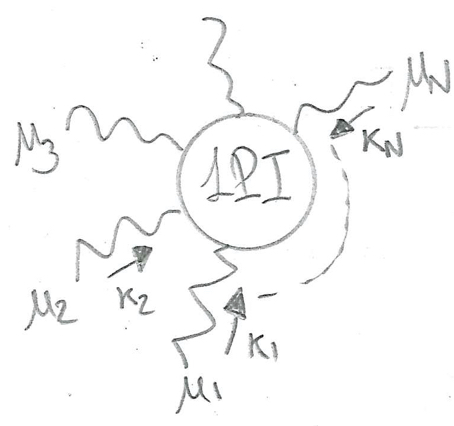
\includegraphics{images_ch4/nphotons_diagr.jpeg} \\ Diagramma ad N fotoni a cui fa riferimento la (\ref{eq:WT_ID_Nphotons}).} e denominiamolo 
    \(iV_N^{\mu_1,...,\mu_N}(k_1,...,k_N)\). Allora 
    \begin{equation}
        \boxed{\begin{aligned} 
            &(k_i)_{\mu_i}V_N^{\mu_1,..., \mu_i, ...,\mu_N}(k_1,...,k_N) =0 \\
            &\forall i = 1,...,N
        \end{aligned}}
        \label{eq:WT_ID_Nphotons}
    \end{equation}
\end{theorem}
I fotoni possono essere anche off-shell, i.e. non è necessario che valga $k_i^2 = 0$.

Inoltre la (\ref{eq:WT_ID_Nphotons}) vale ad ogni ordine in teoria delle perturbazioni.

\subsection{$2$ elettroni; $N$ fotoni.}
\begin{theorem}
    \marginnote{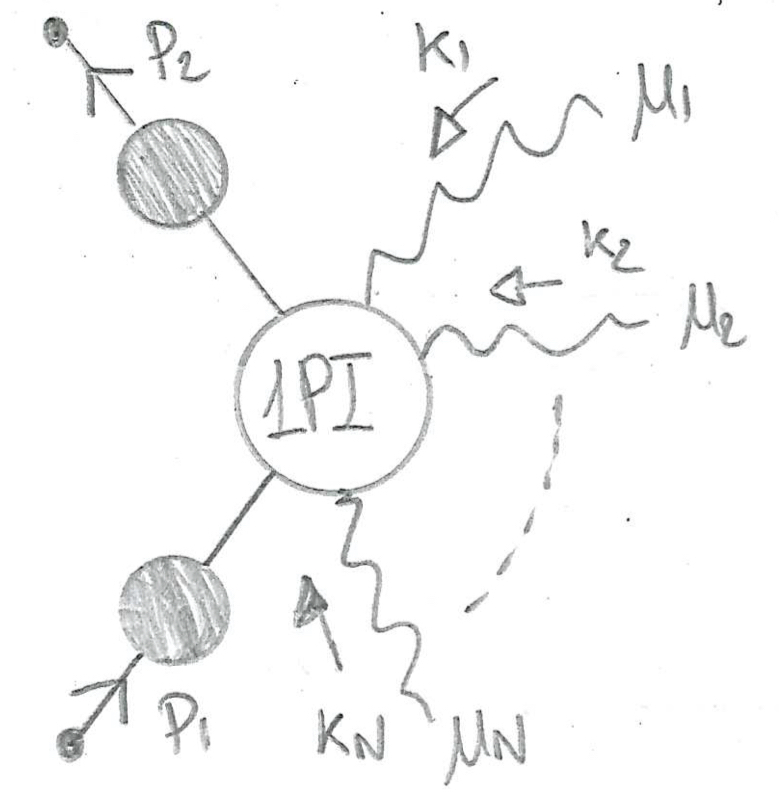
\includegraphics[]{images_ch4/2electr_nphotons_diagr.jpeg}\\ Diagramma con 2 elettroni ed N fotoni a cui fa riferimento la (\ref{eq:WT_ID_2electr_Nphotons}).}
    Consideriamo un diagramma come quello a lato e denominiamolo 
    \[S_N^{\mu_1,...,\mu_N}(p_2,p_1: k_1, ... , k_N) \equiv S_N^{1,...,N}(p_2,p_1)\]
    Allora \(\forall i\)
    \begin{equation}
        \boxed{
        \begin{aligned}
            (k_i)_{\mu_i}S_N^{1,...,N}(p_2,p_1) = &eS_{N-1}^{1,...,\cancel i, ...,N}(p_2,p_1 + k_i) \\
            &- eS_{N-1}^{1,...,\cancel i, ...,N}(p_2 - k_i,p_1)
        \end{aligned}}
        \label{eq:WT_ID_2electr_Nphotons}
    \end{equation}
\end{theorem}
Includiamo i propagatori sulle linee fermioniche, mentre non lo facciamo su quelle fotoniche, che di fatto sono amputate.

Gli impulsi dei fotoni sono entranti, ergo abbiamo
\[p_1 + k_1 + \cdots + k_n = p_2 \Rightarrow \boxed{p_2 - p_1 = k_1 + \cdots + k_n} \]
\paragraph{Dimostrazione diagrammatica della (\ref{eq:WT_ID_2electr_Nphotons}).} Lavoriamo all'ordine più basso in teoria delle perturbazioni.
\begin{itemize}
    \item Dimostriamo che la (\ref{eq:WT_ID_2electr_Nphotons}) è vera al tree-level.\\
    \underline{Consideriamo il caso con N=1}
    \begin{align*}
        \begin{tikzpicture}[baseline=\plusheight]
          \begin{feynman}[] % dressed electron propagator diagram
              \vertex[small, dot] (a) at (-1,0) {} ;
              \vertex[small, dot] (m) at (0,0) {};
              \vertex[small, dot] (b) at (1,0) {};
              \vertex (c) at (0,1) {};
              \diagram*[small] {
                (a)--[anti fermion, edge label'=$p_2$] (m) --[anti fermion, edge label'=$p_1$] (b),
                (c) --[photon, momentum=\(k\)] (m)};
          \end{feynman}
        \end{tikzpicture} 
        \equiv S_1^\mu(p_2,p_1) = \frac{i}{\slashed p_2 - m + i\varepsilon}(ie\gamma^\mu)\frac{i}{\slashed p_1 - m + i\varepsilon}
    \end{align*}
    Adesso contraiamo l'indice $\mu$ con l'impulso dell'unico fotone esterno, per cui ricordiamo valere la relazione \(k=p_2-p_1\)
    \begin{align*}
    k_\mu S_1^\mu(p_2,p_1) & = (-ie)\frac{1}{\slashed p_2 - m + i\varepsilon}\slashed k \frac{1}{\slashed p_1 - m + i\varepsilon}\\
    & = (-ie)\frac{1}{\slashed p_2 - m + i\varepsilon}\bigl(\slashed p_2 - \slashed p_1 + m - m \bigr)\frac{1}{\slashed p_1 - m + i\varepsilon}\\
    &= (-ie)\frac{1}{\slashed p_2 - m + i\varepsilon}\Bigl[\bigl(\slashed p_2 - m\bigr) -\bigl(\slashed p_1 - m\bigr)\Bigr]\frac{1}{\slashed p_1 - m + i\varepsilon} \overset{\star}{=}
    \end{align*}
    A questo punto svolgiamo i prodotti, trascurando quando necessario il fattore $i\varepsilon$ a denominatore per semplificare il numeratore.
    \begin{align*}
    &\overset{\star}{=}-e\frac{i}{\slashed p_1 - m + i\varepsilon} + e \frac{i}{\slashed p_2 - m + i\varepsilon}\\
    &=-eS_0(p_1,p_1) +eS_0(p_2,p_2)
    \end{align*}
    In definitiva:
    \[
    \boxed{
    k_\mu S_1^\mu(p_2,p_1) = eS_0(p_2,p_1 + k) - eS_0(p_2 - k,p_1)}
    \]
    \item Ragionando allo stesso modo per \underline{il caso con N=2}, che coinvolge i diagrammi seguenti (con $q_2 = p_2- k_1$ e $q_1 = p_1 + k_1$)
    \[
    \begin{aligned}
    S_2^{\mu\nu}(p_2,p_1;k_2,k_1)=
    \begin{tikzpicture}[baseline=\plusheight]
        \begin{feynman}
            \vertex[small, dot] (a) at (-1,0) {} ;
            \vertex[small, dot, label=below:$\mu$] (m1) at (0,0) {};
            \vertex[small, dot, label=below:$\nu$] (m2) at (1,0) {};
            \vertex[small, dot] (b) at (2,0) {};
            \vertex (p1) at (0,1) {};
            \vertex (p2) at (1,1) {};
            \diagram*[small]{
                (a) --[anti fermion, edge label'=$p_2$] (m1) --[anti fermion, edge label'=$q_2$] (m2) --[anti fermion, edge label'=$p_1$] (b),
                (p1) --[photon, momentum'=$k_1$] (m1),
                (p2) --[photon, momentum=$k_2$] (m2)
            };
        \end{feynman}
    \end{tikzpicture}
    +
    \begin{tikzpicture}[baseline=\plusheight]
        \begin{feynman}
            \vertex[small, dot] (a) at (-1,0) {} ;
            \vertex[small, dot, label=below:$\nu$] (m1) at (0,0) {};
            \vertex[small, dot, label=below:$\mu$] (m2) at (1,0) {};
            \vertex[small, dot] (b) at (2,0) {};
            \vertex (p1) at (0,1) {};
            \vertex[empty dot,minimum size=0mm] (dummy) at (0.5,0.5) {};
            \vertex (p2) at (1,1) {};
            \diagram*[small]{
                (a) --[anti fermion, edge label'=$p_2$] (m1) --[anti fermion, edge label'=$q_1$] (m2) --[anti fermion, edge label'=$p_1$] (b),
                (p1) --[photon, momentum=$k_1$] (dummy) -- [photon] (m2),
                (p2) --[photon, momentum=$k_2$] (dummy) -- [photon] (m1)
            };
        \end{feynman}
    \end{tikzpicture}
    \end{aligned}\]
    da cui segue 
    \begin{align*}
    S_2^{\mu\nu}(p_2,p_1;k_2,k_1) = &\frac{i}{\slashed p_2 - m}(ie\gamma^\mu)\frac{i}{\slashed p_2 - \slashed k_1 - m}(ie\gamma^\nu)\frac{i}{\slashed p_1 - m} \\
    &+ \frac{i}{\slashed p_2 - m}(ie\gamma^\nu)\frac{i}{\slashed p_1 + \slashed k_1 - m}(ie\gamma^\mu)\frac{i}{\slashed p_1 - m}
    \end{align*}
    e calcolando la contrazione \((k_1)_\mu S_2^{\mu\nu}(p_2,p_1;k_2,k_1)\) con più o meno le stesse tecniche di prima [\textbf{conti svolti lezione 12, pag.44÷45}], si arriva al risultato:
    \[ \boxed{(k_1)_\mu S_2^{\mu\nu}(p_2,p_1;k_2,k_1) = eS_1^{\nu}(p_2,p_1+k_1;k_2) - eS_1^{\nu}(p_2-k_1,p_1;k_2)} \]

    Per induzione matematica segue il risultato generale. \qed
\end{itemize}
Torniamo adesso al caso precedente.
\paragraph{Dimostrazione diagrammatica della (\ref{eq:WT_ID_Nphotons}).}\marginnote{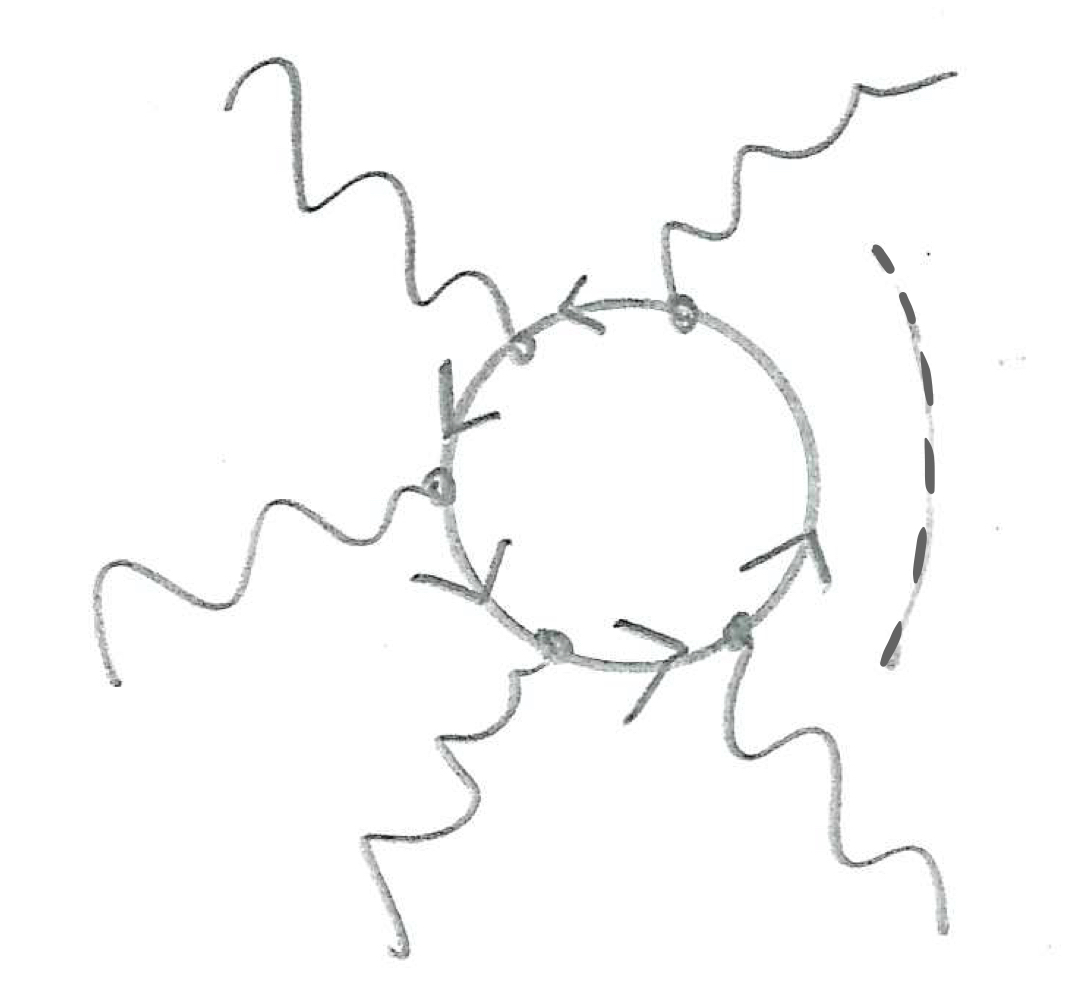
\includegraphics[]{images_ch4/nphotons_diagr_1loop.jpeg}}
Lavoriamo ad un loop e consideriamo il diagramma con $N$ fotoni a lato e tutte le sue permutazioni e chiamiamolo \(iV_{N, \text{1-loop}}^{1,...,N}\).

Il calcolo di questo loop coinvolge una traccia e dobbiamo sommare su tutte le permutazioni. Inoltre si dimostra che con $N$ fotoni, il numero di contrazioni non equivalenti è pari a $(N-1)!$

Va notato come ogni contributo proveniente da una permutazione coinvolge una traccia, quindi usando la ciclicità sarà sempre possibile tenere un determinato fotone (e quiondi il suo relativo contributo al vertice) all'inizio.

\underline{Consideriamo il caso specifico con $N=3$}. Dobbiamo considerare i seguenti diagrammi, dove utilizziamo \(q_3 = p+k_1+k_3\) e \(q_2 = p+k_1+k_2\):
\marginnote{Osserviamo che il diagramma con i fotoni scambiati è equivalente a quello con i fermioni che vanno in direzione opposta nel loop}
\begin{align*}
    iV_{3, \text{1-loop}}^{\mu\nu\rho} = 
    \feynmandiagram [small, horizontal=a to t1, inline=(a.base)] {
        a [particle=\(\mu\)] -- [photon, momentum=\(k_1\)] t1[small, dot] --[fermion, edge label'=\(p+k_1\)] t2[small, dot] --[fermion, edge label'=\(q_3\)] t3[small, dot] --[fermion, edge label'=\(p\)] t1,
        p1 [particle=\(\rho\)] -- [photon, momentum=\(k_3\)] t2 ,
        p2 [particle=\(\nu\)] -- [photon, momentum'=\(k_2\)] t3  ,
        p1 -- [opacity=0] p2,
        };
        +
    \begin{tikzpicture}[baseline=\plusheight]
        \begin{feynman}
        \diagram[small, horizontal=a to t1] {
            a [particle=\(\mu\)] -- [photon, momentum=\(k_1\)] t1[small, dot] --[fermion, edge label'=\(p+k_1\)] t2[small, dot] --[fermion, edge label'=\(q_2\)] t3[small, dot] --[fermion, edge label'=\(p\)] t1,
            p1 [particle=\(\rho\)] -- [draw=none] t2 ,
            p2 [particle=\(\nu\)] -- [draw=none]  t3  ,
            p1 -- [opacity=0] p2,
            };
        \diagram*{
        (p1) -- [photon] (t3) ,
        (p2) -- [photon] (t2),
        };
        \end{feynman}
    \end{tikzpicture}
\end{align*}

A questo punto non è difficile accorgersi del fatto che il calcolo di questi diagrammi riproduce all'interno della traccia la stessa struttura di \(S_2^{\nu\rho}(p, p+k_1)\), moltiplicata a sinistra per \(ie\gamma^\mu\).

In sostanza stiamo dicendo che 
\[
iV_{3, \text{1-loop}}^{\mu\nu\rho} = \int\frac{d^4p}{(2\pi)^4}(-1)\Tr{(ie\gamma^\mu)
S_2^{\nu\rho}(p, p+k_1)}
\]
Quanto appena visto è vero in generale e possiamo scrivere diagrammaticamente:

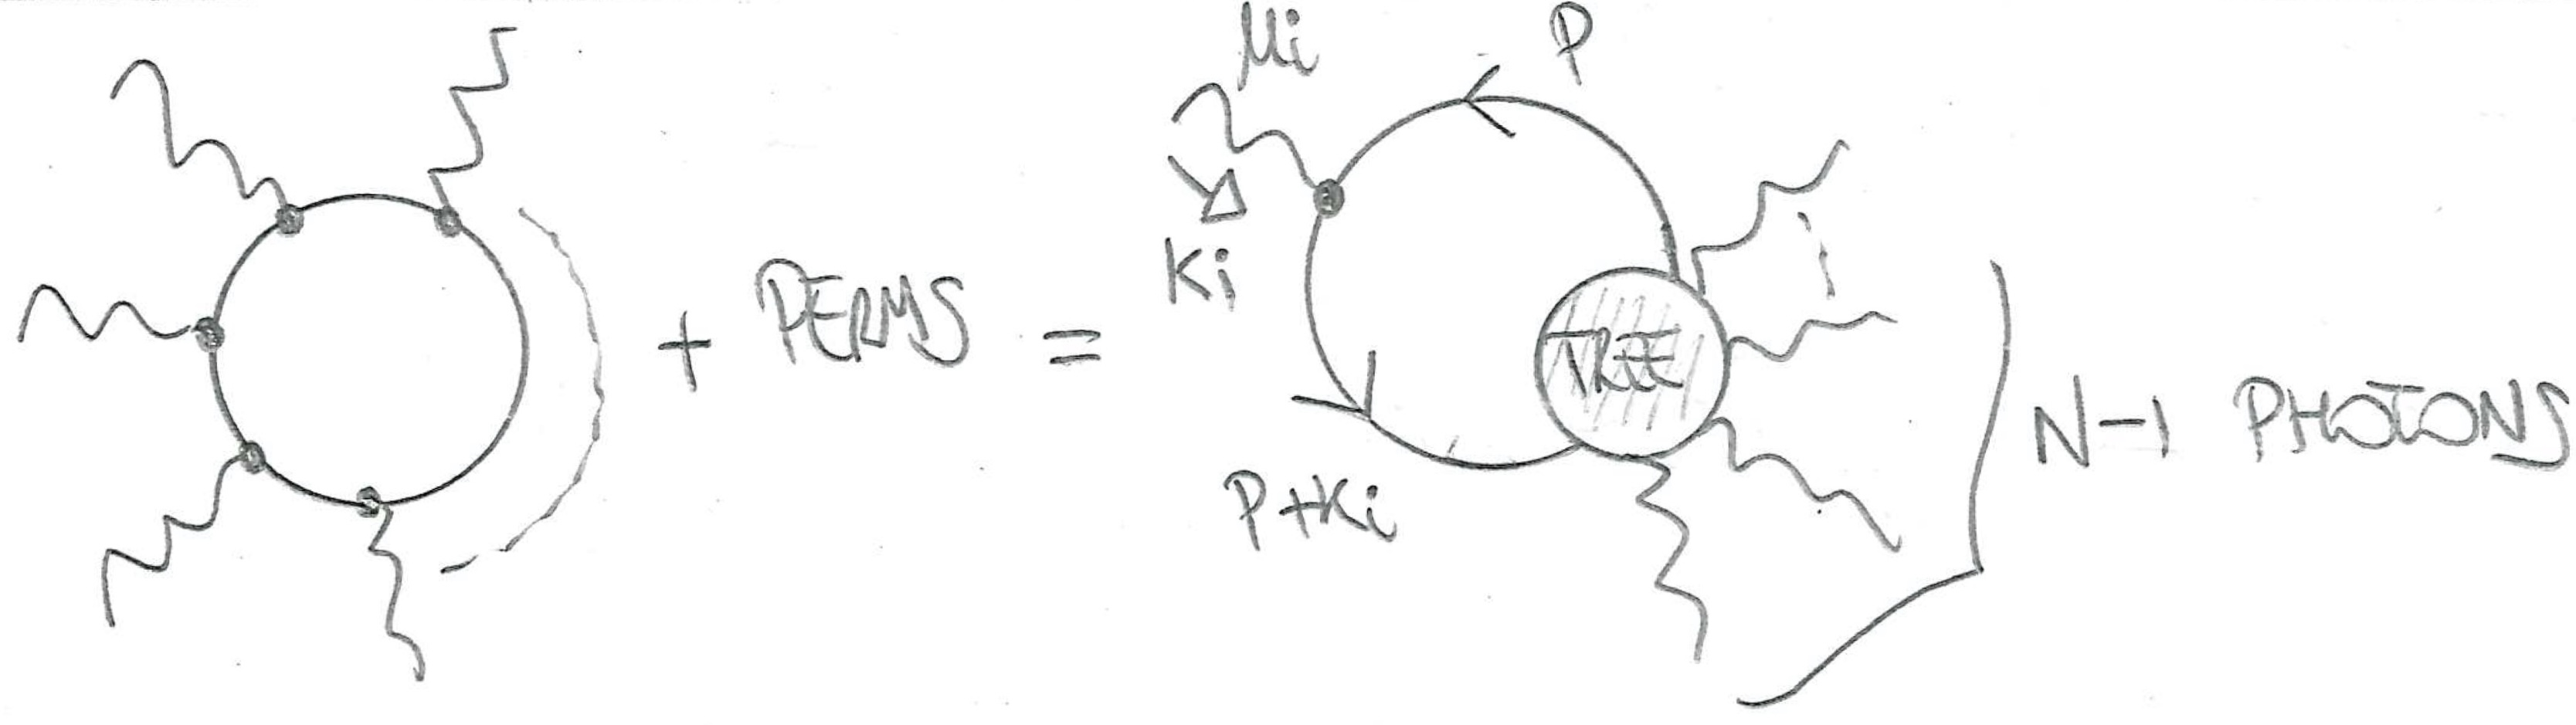
\includegraphics[]{images_ch4/nphotons_diagr_1loop_general.jpg}

che corrisponde all'equazione:
\begin{equation}
    iV_{N, \text{1-loop}}^{1,...,N} = \int\frac{d^4p}{(2\pi)^4}(-1)\Tr{(ie\gamma^{\mu_i})S_{N-1}^{1,..,\cancel{i},..,N}(p, p+k_i) }
\end{equation}

Contraiamo ora con un certo $k_j$ e troviamo:

\[(k_j)_{\mu_j}iV_{N, \text{1-loop}}^{1,...,N} = \int\frac{d^4p}{(2\pi)^4}(-1)\Tr{(ie\gamma^{\mu_i})(k_j)_{\mu_j}S_{N-1}^{1,..,\cancel{i},..,N}(p, p+k_i) }\]

A questo punto utilizziamo l'identità (\ref{eq:WT_ID_2electr_Nphotons}) 
\begin{align*}
    (k_j)_{\mu_j}iV_{N, \text{1-loop}}^{1,...,N} = &-\int\frac{d^4p}{(2\pi)^4}\Tr{(ie\gamma^{\mu_i})(k_j)_{\mu_j}eS_{N-2}^{1,..,\cancel{j},..,\cancel{i},..,N}(p, p+k_i+k_j) } \\
    &+ \int\frac{d^4p}{(2\pi)^4}\Tr{(ie\gamma^{\mu_i})(k_j)_{\mu_j}eS_{N-2}^{1,..,\cancel{j},..,\cancel{i},..,N}(p-k_j, p+k_i) }
\end{align*}
Cambiamo variabile di integrazione prendendo \(p=p+k_j\) (e quindi \(p + k_i=p+k_j+k_i\)) ed il gioco è fatto: i due termini sono uguali a meno del segno ed abbiamo verificato che 
\[
(k_j)_{\mu_j}iV_{N, \text{1-loop}}^{1,...,N} = 0
\]\qed

\begin{nota}
    Queste identità, giustificate diagrammaticamente all'ordine minore, sono valide in maniera non perturbativa, i.e. sono esatte.
\end{nota}

\subsection{Implicazioni delle WTI}
\subsubsection{\(\mathbf{Z_1 = Z_2}\)}

Consideriamo il vertice di interazione in cui includiamo i propagatori vestiti fermionici e lavoriamo con la Lagrangiana nuda. Con la notazione che abbiamo introdotto prima possiamo denominarlo nel modo seguente:
\[
    \begin{tikzpicture}[baseline=\plusheight]
        \begin{feynman}
            \vertex[dot] (a) at (-1,-1) {};
            \vertex[blob, minimum size=3mm] (bloba) at (-0.5,-0.5) {};
            \vertex[dot] (b) at (-1,1) {};
            \vertex[blob, minimum size=3mm] (blobb) at (-0.5,0.5) {};
            \vertex[blob, fill=white!100, minimum size=7mm] (v) at (0,0) {1PI};
            \vertex[label=below:\(\mu\)] (c) at (1.5,0) {};
            \diagram*[small]{
                (a) -- [fermion, edge label=\(p_1\)] (bloba) -- (v) -- (blobb) --[fermion, edge label=\(p_2\)] (b),
                (c) --[photon, momentum'=\(q\)] (v)  
            };
        \end{feynman}
    \end{tikzpicture}
    = S_1^\mu(p_2,p_1;q)
\]
Allo stesso tempo possiamo rinominare anche il propagatore vestito fermionico, uniformandoci alla notazione, che quindi diventa:
\[
\feynmandiagram[horizontal=a to b, small, layered layout, inline=(b.base)]{
    a[dot] --[fermion,edge label=\(p\)] v[blob, minimum size=8mm] --[fermion] b[dot]
};
= \frac{i}{\slashed p - m_B + \Sigma(\slashed p) + i\epsilon} \equiv S_0(p)
\]
Di conseguenza il diagramma del vertice di interazione può essere scritto come segue:
\begin{equation}
    { S_1^\mu(p_2,p_1;q) = S_0(p_2)\bigl[ ie_B\Gamma^\mu(p_1,p_2) \bigr] S_0(p_1) }
    \label{eq:vertex_function_newnotation}
\end{equation}

A questo punto contraiamo con $q_\mu$ applicando la (\ref{eq:WT_ID_2electr_Nphotons}) al LHS della (\ref{eq:vertex_function_newnotation}):
\marginnote{Applicando l'identità di W-T, scompare la dipendenza da $p_1$ e $p_2$, rispettivamente, nei due termini in cui separiamo $S_1^\mu$. 

Questo è conseguenza della conservazione dell'impulso: infatti che $q=p_2-p_1$ per costruzione, e per la (\ref{eq:WT_ID_2electr_Nphotons}) ad RHS abbiamo le dipendenze $p_1+q=p_2$ e $p_2-q=p_1$, rispettivamente, nei due termini, che quindi sono ripetute.}
\begin{align*}
    q_\mu S_1^\mu(p_2,p_1;q) &= ie_B S_0(p_2) q_\mu \Gamma^\mu(p_1,p_2) S_0(p_1)\\
                             &\overset{!}{=} e_B S_0(p_2) - e_B S_0(p_1)
\end{align*}

Adesso lavoriamo sulla seconda uguaglianza, possiamo semplificare la carica e risolvere per \(iq_\mu\Gamma^\mu\), per poi sostituire l'espressione esplicita del propagatore vestito (inverso), trovando:
\begin{align*}
    iq_\mu\Gamma^\mu(p_2,p_1) &= S_0(p_1)^{-1} - S_0(p_2)^{-1} \\
                    &= (-i)\bigl[\slashed p_1 - m_B + \Sigma(\slashed p_1) \bigr] +i\bigl[\slashed p_2 - m_B + \Sigma(\slashed p_2) \bigr]\\
                    &=i\bigl[\slashed p_2 - \cancel{m_B} + \Sigma(\slashed p_2) -\slashed p_1 + \cancel{m_B} - \Sigma(\slashed p_1) \bigr]
\end{align*}

Otteniamo quindi quello che rappresenta l'identità di Ward-Takahashi per il fotone entrante:
\begin{equation}
    q_\mu\Gamma^\mu(p_2,p_1) = \overbrace{\slashed p_2 -\slashed p_1}^{\slashed q} + \Sigma(\slashed p_2)  - \Sigma(\slashed p_1)
    \label{eq:entering_photon_contraction}
\end{equation}
ora prendiamone il limite per $q\rightarrow 0 \Rightarrow p_2=p_1$ ed espandiamo $\Sigma(\slashed p_2)$ nell'intorno $\slashed p_2 = \slashed p_1$, considerando inoltre i fermioni on-shell ($p_2^2 = p_1^2 = m^2_\text{phys}$):
\begin{align*}
    \lim_{q\rightarrow 0}q_\mu\Gamma^\mu(p_2,p_1) &= \slashed q + \cancel{\Sigma(\slashed p_1)} + \frac{d\Sigma(\slashed p)}{d\slashed p}\bigg|_{\slashed p_1}(\slashed p_2-\slashed p_1)-\cancel{\Sigma(\slashed p_1)}\\
        &= \underbrace{\biggl[1+ \frac{d\Sigma(\slashed p)}{d\slashed p}\bigg|_{m_\text{phys}}\biggr]}_{=Z_2^{-1}}\slashed q = \frac{\gamma^\mu q_\mu}{Z_2} \\
\end{align*}

In definitiva troviamo:
\begin{equation}
    \boxed{\Gamma^\mu(\text{on-shell } p_1=p_2) = \frac{\gamma^\mu}{Z_2}}
    \label{eq:Gamma_mu_scale}
\end{equation}
Consideriamo ora la definizione di carica elettrica (\ref{def:electric_charge}), lavorando sempre nella teoria nuda.

Vogliamo quindi valutare l'ampiezza del processo:
\[
    \begin{tikzpicture}[baseline=\plusheight]
        \begin{feynman}
            \vertex (a) at (-1,-1) {};
            \vertex (b) at (-1,1) {};
            \vertex[blob, fill=white!100] (v) at (0,0) {1PI};
            \vertex (c) at (1.5,0) {};
            \diagram*[small]{
                (a) -- [fermion, edge label'=\(p_1\)] (v) --[fermion, edge label'=\(p_2\)] (b),
                (v)--[photon, momentum=\(q\)] (c) 
            };
        \end{feynman}
    \end{tikzpicture}
\]
che può essere scritta, utilizzando i formalismi introdotti in sezione \ref{sec:poles_formal_discussion}:
\[
i\mathcal{M} = \bar u(p_2)Z_2ie_B\Gamma^\mu(p_1,p_2) u(p_1) \sqrt{Z_3} \varepsilon^*_\mu(q)
\]
Nel limite di $q\rightarrow0$ possiamo applicare la definizione di carica elettrica al diagramma, ottenendo la seguente uguaglianza

\[
\bar u(p_2)Z_2ie_B\Gamma^\mu(p_1,p_2) u(p_1) \sqrt{Z_3} \varepsilon^*_\mu(q) \overset{q\rightarrow0}{=} \bar u(p_2)ie_\text{phys}\gamma^\mu u(p_1)\varepsilon^*_\mu(q)
\]
da cui segue che 
\[
e_\text{phys}\gamma^\mu = e_B \underbrace{\Gamma^\mu(p_1,p_2) Z_2}_{\overset{\text{\ref{eq:Gamma_mu_scale}}}{=}\gamma^\mu} \sqrt{Z_3} = e_B\gamma^\mu\sqrt{Z_3}
\]
Abbiamo quindi trovato quella che viene definita \textbf{(Universalità del coupling rinormalizzato di QED)}:
\begin{equation}
    \boxed{e_\text{phys} = \sqrt{Z_3} e_B}
\end{equation}

Ora ricordiamo la relazione tra carica nuda e rinormalizzata:
\[e_B = Z_e e_R = \frac{Z_1}{Z_2\sqrt{Z_3}}e_R\]
Siccome nello schema On-Shell \(e_R = e_\text{phys} \), troviamo ciò che avevamo già trovato trattando esplicitamente la rinormalizzazione del vertice di interazione, passando per i controtermini, in sezione \ref{sec:vertex_renorm}:

\[e_B = \frac{Z_1}{Z_2\sqrt{Z_3}}(\sqrt{Z_3}e_B) \Rightarrow \boxed{Z_1=Z_2}\]

\subsubsection{L'identità di Ward}
Consideriamo l'identità di Ward-Takahashi (\ref{eq:WT_ID_2electr_Nphotons}), che equivale, dal punto di vista diagrammatico, a:

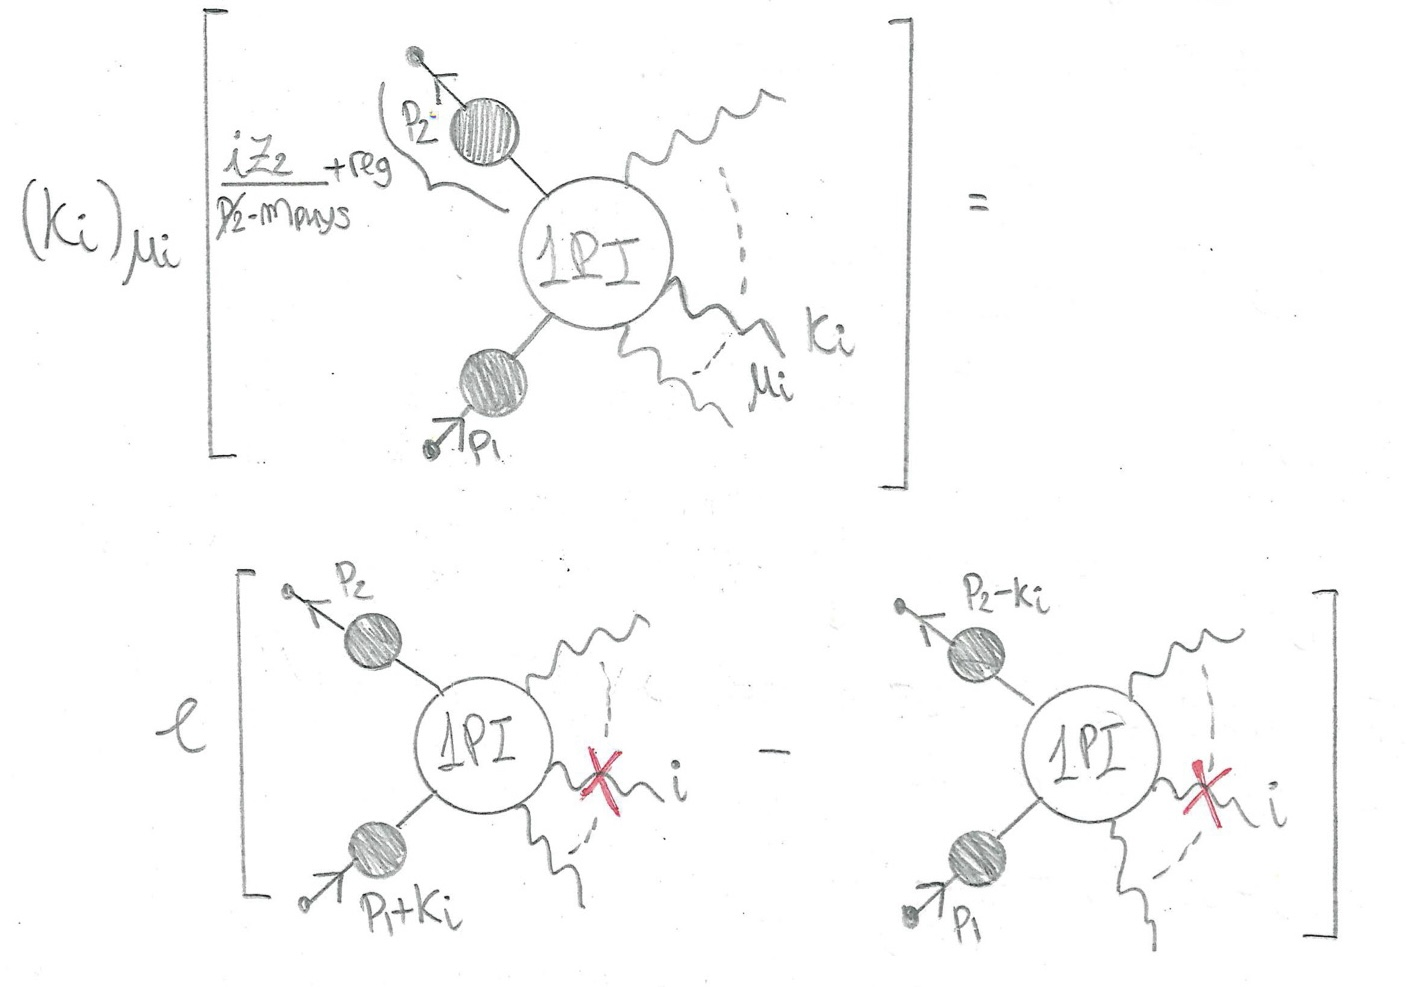
\includegraphics[width=\linewidth]{images_ch4/WT_ID_2elctr_Nphot.jpg}

Vorremmo \textit{convertire questa identità in un identità per le ampiezze di scattering}. A tal scopo amputiamo le linee fermioniche esterne per mezzo del procedimento di riduzione LSZ.

In altre parole moltiplichiamo per \( (\slashed p_1 - m_\text{phys})(\slashed p_2 - m_\text{phys}) \) e prendiamo il limite on-shell \(p_1^2=p_2^2=m^2_\text{phys}\).

Al LHS dell'identità questo step riproduce l'ampiezza di scattering con due fermioni on-shell, siccome i propagatori esterni hanno poli semplici precisamente in \(\slashed p_{1,2} = m_\text{phys}\).

Tuttavia, al RHS gli impulsi sulle gambe esterne non coincidono, ed entrambi i termini andranno a zero nel limite \(\slashed p_{1,2} = m_\text{phys}\).

Arriviamo quindi al seguente teorema
\begin{theorem}
    \textbf{(Identità di Ward.)}
    \marginnote{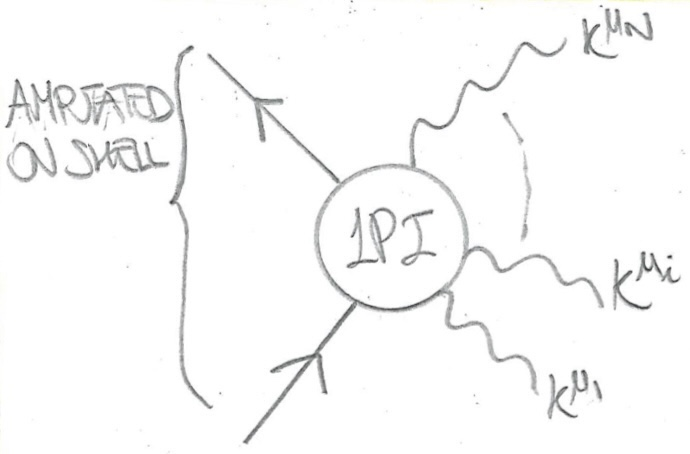
\includegraphics[]{images_ch4/Ward_identity.jpg}}

    Considerato un diagramma ad $N$ fotoni (non necessariamente on-shell) ed arbitrario numero di fermioni (necessariamente on shell ed amputati) come quello a margine, che identifichiamo con l'ampiezza \(i\mathcal{M}^{\mu_1,...,\mu_N}\).

    Contraendo tale ampiezza con un impulso $k_{\mu_i}$ di uno dei fotoni partecipanti al diagramma, tale contrazione risulta nulla, ovvero:
    
    \begin{equation}
        \boxed{k_{\mu_i}\mathcal{M}^{\mu_1,..,\mu_i,..,\mu_N} = 0}
        \label{eq:ward_id_formal}
    \end{equation}
    \label{th:Ward_identity}
\end{theorem}

\end{document}
